
\section{یادگیری بدون ناظر}
    در مطالعه علوم اعصاب محاسباتی، درک مکانیسم‌های پلاستیسیته سیناپسی
    \footnote{\lr{synaptic plasticity}}
    - چگونگی تقویت یا تضعیف ارتباطات بین نورون‌ها در طول زمان، که از آن به عنوان یادگیری نیز یاد می‌شود - بسیار مهم است. یکی از مدل‌های اصلی برای شبیه‌سازی یادگیری در مغز، قانون یادگیری انعطاف‌پذیری وابسته به زمان ضربه 
    ($STDP$ \footnote{Spike-Timing-Dependent Plasticity})
    است. این مدل به عنوان یک چارچوب ساده ولی قوی برای بررسی چگونگی تأثیر زمان ضربه ها در ارتباطات عصبی بر ارتباطات سیناپسی، در نتیجه یادگیری و حافظه در شبکه‌های عصبی مغز قرار می‌گیرد.

    $STDP$
    یک فرآیند بیولوژیکی است که قدرت اتصالات بین نورون های مغز را تنظیم می کند. این فرآیند، نقاط قوت اتصال را بر اساس زمان‌بندی نسبی خروجی یک نورون خاص و پتانسیل‌های عمل ورودی 
    (یا ضربه)
    تنظیم می‌کند.

    در فرآیند 
    $STDP،$، 
    اگر یک ضربه ورودی به یک نورون، به طور متوسط، بلافاصله قبل از ضربه خروجی آن نورون رخ دهد، آن ورودی خاص تا حدودی قوی‌تر می‌شود. اگر یک ضربه ورودی، به طور متوسط، بلافاصله پس از یک ضربه خروجی رخ دهد، آن ورودی خاص تا حدودی ضعیف‌تر می‌شود، بنابراین معنای «یادگیری انعطاف‌پذیری وابسته به زمان ضربه» برای ما روشن تر می شود. بنابراین، ورودی‌هایی که ممکن است علت برانگیختگی نورون پس سیناپسی باشند، احتمالاً در آینده کمک می‌کنند، در حالی که ورودی‌هایی که علت ضربه پس سیناپسی نیستند، کمتر در آینده کمک می‌کنند. این فرآیند تا زمانی ادامه می‌یابد که زیرمجموعه‌ای از مجموعه اولیه اتصالات باقی می‌ماند، در حالی که تأثیر همه اتصالات دیگر به 0 کاهش می‌یابد.
    \cite{STDP-Wikipedia}
    از آنجایی که یک نورون زمانی که بسیاری از ورودی‌هایش در یک دوره کوتاه اتفاق می‌افتند یک ضربه خروجی تولید می‌کند، زیرمجموعه ورودی‌هایی که باقی می‌مانند عبارتند از آنهایی که تمایل به همبستگی در زمان داشتند. علاوه بر این، از آنجایی که ورودی‌هایی که قبل از خروجی تقویت می‌شوند، ورودی‌هایی که اولین نشانه‌های همبستگی را ارائه می‌دهند، در نهایت به ورودی نهایی نورون تبدیل می‌شوند.

    $STDP$ 
    خود به چندین مدل میتواند پیاده سازی شود که از بین این مدل ها، مدل 
    \lr{Pair-based STDP wtih local variables}
    برای بررسی انتخاب شده است.

    \subsection{\lr{Pair-based STDP}}
        در مدل 
        $STDP$ 
        مبتنی بر جفت، تنظیم وزن های سیناپسی با لحظه‌های دقیق وقوع ضربه در نورون‌های پیش سیناپسی و پس سیناپسی انجام می‌شود. این مدل از دو متغیر محلی - اثر
        \footnote{trace}
        ضربه پیش سیناپسی و اثر ضربه پس سیناپسی - برای ثبت تاریخچه ضربه عصبی استفاده می کند که بر تغییرات سیناپسی تأثیر می گذارد.

        \begin{itemize}
            \item \textbf{اثر ضربه پیش سیناپسی $x_j$:}
                این اثر در طول زمان با یک ثابت کاهشی، کاهش می‌یابد اما با هر ضربه پیش سیناپسی دوباره افزایش می‌یابد و به طور موثر زمان این ضربه ها را مشخص می‌کند. نحوه بروزرسانی این مقدار توسط فرمول زیر می تواند محاسبه شود:
                \begin{equation}
                    \frac{dx_j}{dt} = -\frac{x_j}{\tau_+} + \sum_{f}\delta(t-t_{j}^{f})
                \end{equation}
            \item \textbf{اثر ضربه پس سیناپسی $y_i$:}
            مشابه اثر پیش سیناپسی، این اثر نیز در طول زمان تحلیل می‌رود، اما با ضربه پس سیناپسی افزایش می‌یابد.  نحوه بروزرسانی این مقدار توسط فرمول زیر می تواند محاسبه شود:
            \begin{equation}
                \frac{dy_i}{dt} = -\frac{y_i}{\tau_-} + \sum_{f}\delta(t-t_{i}^{f})
            \end{equation}
        \end{itemize}

        این اثر ها
        (ردپاها)
        بسیار مهم هستند زیرا مبنایی برای محاسبه تغییرات سیناپسی بلافاصله پس از ضربه زدن هستند و باعث می‌شود که مدل به زمان ضربه پاسخ دهد.

        سپس نوبت به تغییرات وزن ها میرسد. این تغییرات بر اساس مقادیر فعلی اثر های گفته شده در هر زمان که یک ضربه زده می شود محاسبه می شود. این روش نه تنها با مشاهدات بیولوژیکی هماهنگ است، بلکه امکان شبیه سازی دقیق فرآیندهای یادگیری و تشکیل حافظه در شبکه را نیز فراهم می کند. نحوه بروزرسانی وزن ها نیز توسط فرمول زیر امکان پذیر است:
        \begin{equation}
            \frac{dw_{ij}}{dt} = -A_{-}(w_{ij})y_{i}(t)\sum_{f}\delta(t-t^{f}_{j})+A_{+}(w_{ij})x_{j}(t)\sum_{f}\delta(t-t^{f}_{i})
        \end{equation}

        قبل از رفتن به آزمایش کردن مدل، یک نکته دیگر باقی می ماند و آن این است که برای 
        $A_{-}$، $A_{+}$ 
        میتواند توابعی
        \footnote{\lr{Soft/Hard bound}}
        برای کنترل کردن محدوده وزن ها استفاده شود.
        
        
    \subsection{آزمایش ها}
        \paragraph*{شباهت کسینوسی:}
            \textbf{ دقت شود که نمودار شباهت کسینوسی در تمام شکل ها آمده است.}

        حال در این قسمت، به سراغ آزمایش مدل 
        $STDP$ 
        مان میرویم و نمودار های خواسته شده در موارد الف تا و را بررسی میکنیم. 
        
        ابتدا دو الگوی به صورت آرایه را به مدل میدهیم. برای اینکار میتوانیم یک آرایه تصادفی از اعداد ۱ تا ۱۰ و یک آرایه تصادفی دیگر که مقادیر آن دوبرابر آرایه اول است را به عنوان ورودی به جمعیت ورودی بدهیم. از این رو، مطابق شکل 
        \ref{fig:part2-small-array-stdp}
        مشاهده میکنیم که با تغییر وزن های سیناپسی، هر نورون یکی از الگو ها را یادگرفته است. به طوری که وقتی الگوی یاد گرفته شده را میبیند نرخ ضربه زدن آن بیشتر می شود.
        \begin{figure}[!ht]
            \centering
            \includegraphics[width=1\textwidth]{plots/part2-small-array-stdp.pdf} 
            \caption{قانون یادگیری 
            $STDP$.
            همانطور که از شکل نیز مشخص است، وزن های سیناپسی طوری تنظیم می شوند که هر نورون، یکی از الگو ها را یاد میگیرد. همچنین طبق نمودار شباهت کسینوسی، به مرور زمان، شباهت بین وزن های دونورون خروجی نیز کاهش می یابد.}
            \label{fig:part2-small-array-stdp}
        \end{figure}

        \subsubsection*{تغییر در اندازه ورودی}
        هر چند این یادگیری به دلیل بدون ناظر بودن شبکه و همچنین ساده بودن آن، از عهده یادگیری الگو های پیچیده تر ممکن است برنیاید. به طور مثال، با زیاد کردن طول آرایه، ویژگی های مورد نیاز برای تشخیص دادن نیز افزایش یافته پیداست، یادگیری ممکن است به خوبی انجام نشود. به عنوان مثال، در شکل 
        \ref{fig:part2-large-array-stdp}
        یادگیری به خوبی انجام شده است، ولی نسبت به شکل 
        \ref{fig:part2-small-array-stdp} 
        دیرتر یادگیری شکل گرفته است.

        \begin{figure}[htbp]
            \centering
            \includegraphics[width=1\textwidth]{plots/part2-large-array-stdp.pdf} 
            \caption{قانون یادگیری 
            $STDP$ برای ورودی بزرگتر.
            مطابق شکل ملاحظه میکنیم علی رغم اینکه مدل توانسته تا تکرار ۱۰۰۰ ام شبیه سازی به خوبی الگو ها را یاد بگیرد، ولی نسبت به شکل
            \ref{fig:part2-small-array-stdp}
            که ورودی کوچکتر بود این اتفاق دیرتر افتاده است. هرچند با تغییر پارامتر هایی مانند پنجره زمانی یا نرخ یادگیری می‌توان این یادگیری را سریع تر انجام داد که این موضوع را در ادامه بررسی خواهیم کرد.}
            \label{fig:part2-large-array-stdp}
        \end{figure}
        
        حال مطابق خواسته پروژه، ورودی ها را به گونه‌ای به شبکه می‌دهیم که نورون های ورودی در دریافت محرک هم‌پوشانی داشته باشند. یعنی بعضی نورون ها، مسئول گرفتن هر دو ورودی باشند. 
        (مطابق شکل \ref{fig:part2-input-overlap})
        \begin{figure}[!ht]
            \centering
            \captionsetup{width=.9\linewidth}
            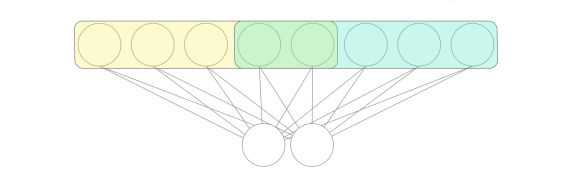
\includegraphics[width=0.9\textwidth]{images/input-overlap.png} 
            \caption{نورون هایی که با رنگ سبز مشخص شده اند، هر دو الگو را به عنوان ورودی دریافت میکنند.
            }
            \label{fig:part2-input-overlap}
        \end{figure}

        ابتدا با هم‌پوشانی کم شروع می‌کنیم. مطابق شکل
        \ref{fig:part2-array-stdp-overlap}
        دریافت می شود که هم‌پوشانی نورون ها در دریافت ورودی نمی‌تواند مانع یادگرفتن مدل شود هر چند که سرعت آن را کاهش می‌دهد.
        \begin{figure}[!ht]
            \centering
            \captionsetup{width=.9\linewidth}
            \includegraphics[width=0.9\textwidth]{plots/part2-array-stdp-overlap.pdf} 
            \caption{هم‌پوشانی نسبی نورون های لایه اول برای دریافت ورودی. مطابق شکل ملاحظه میکنیم که هم‌پوشانی بین نورون های ورودی باعث می‌شود یادگیری در زمان کمی دیرتری اتفاق بیوفتد ولی مانع آن نمی‌شود.
            }
            \label{fig:part2-array-stdp-overlap}
        \end{figure}

        حال این هم‌پوشانی را حداکثر میکنیم به طوری که تمام نورون های ورودی مسئول دریافت هر دو الگو باشند. انتظار داریم که افزایش این هم‌پوشانی، منجر به اختلال در یادگیری شود یا یادگیری را به تعویق بیندازد. شکل
        \ref{fig:part2-array-stdp-high-overlap}
        این موضوع را تایید میکند.

        \begin{figure}[!ht]
            \centering
            \captionsetup{width=.9\linewidth}
            \includegraphics[width=0.9\textwidth]{plots/part2-array-stdp-high-overlap.pdf} 
            \caption{هم‌پوشانی کامل نورون های لایه اول برای دریافت ورودی. مطابق شکل ملاحظه میکنیم که هم‌پوشانی کامل بین نورون های ورودی باعث می‌شود یادگیری مختل شود و مثلا در شکل بالا فقط یکی از نورون ها یکی از الگو ها را یاد بگیرد. این به دلیل ساده بودن مدل 
            $STDP$ 
            است. به طوری که در بخش سوم مشاهده میکنیم که مدل 
            $RSTDP$ 
            نسبت به این هم‌پوشانی پایدار است.
            }
            \label{fig:part2-array-stdp-high-overlap}
        \end{figure}
        ممکن است این موضوع که مدلمان می تواند الگو های نظیر آرایه های بالا را تشخیص دهد، کنجکاوی ما را برانگیزد تا بخواهیم الگو های پیچیده تری مانند تصویر را نیز تشخیص دهیم. برای اینکار، ابتدا از الگو های ساده تری مانند تصاویر 
        \ref{fig:part2-pattern1} و 
        \ref{fig:part2-pattern2} 
        استفاده میکنیم تا قدرت مدل را بسنجیم و سپس به سراغ الگو های پیچیده تر می رویم.

        \begin{figure}[!ht]
            \centering
            \captionsetup{width=.9\linewidth}
            \begin{subfigure}[b]{0.35\textwidth}
                \centering
                
\includegraphics[width=\textwidth]{images/pattern1.png}
                \caption{الگوی اول}
                \label{fig:part2-pattern1}
            \end{subfigure}
            \hfill
            \begin{subfigure}[b]{0.35\textwidth}
                \centering
                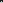
\includegraphics[width=\textwidth]{images/pattern2.png}
                \caption{الگوی دوم}
                \label{fig:part2-pattern2}
            \end{subfigure}
            \caption{دو تصویر به عنوان محرک}
            \label{fig:patterns}
        \end{figure}

        مطابق شکل 
        \ref{fig:part2-pattern-stdp} 
        ملاحظه میکنیم که مدل به خوبی از عهده تشخیص الگو های ساده 
        \ref{fig:part2-pattern1} و 
        \ref{fig:part2-pattern2} 
        برآمد و میتواند آن ها را تشخیص دهد.

        \begin{figure}[htbp]
            \centering
            \includegraphics[width=1\textwidth]{plots/part2-pattern-stdp.pdf} 
            \caption{قانون یادگیری 
            $STDP$ برای ورودی تصویر ساده. 
            مشاهده میکنیم که مدل توانسته به خوبی پ. الگوی تصویری ساده را از یکدیگر تشخیص دهد.
            }
            \label{fig:part2-pattern-stdp}
        \end{figure}

        حال یک قدم فراتر رفته و یک تصویر بزرگتر را به عنوان ورودی به مدل می‌دهیم. ابعاد این تصاویر بزرگتر بوده
        ($10\times 10$) 
        و پیچیده تر هستند. 
        (تصاویر 
        \ref{fig:part2-input-image1} و
        \ref{fig:part2-input-image2})
        \begin{figure}[htbp]
            \centering
            \captionsetup{width=.9\linewidth}
            \begin{subfigure}[b]{0.35\textwidth}
                \centering
                
\includegraphics[width=\textwidth]{images/slop-resized.jpg}
                \caption{تصویر اول}
                \label{fig:part2-input-image1}
            \end{subfigure}
            \hfill
            \begin{subfigure}[b]{0.35\textwidth}
                \centering
                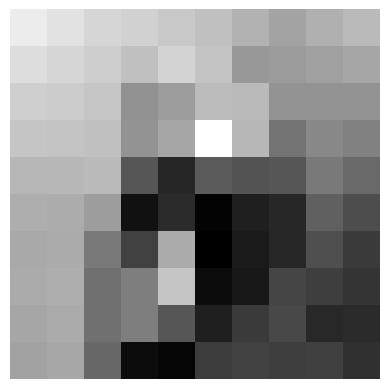
\includegraphics[width=\textwidth]{images/bird-resized.jpg}
                \caption{تصویر دوم}
                \label{fig:part2-input-image2}
            \end{subfigure}
            \caption{یک تصویر به عنوان محرک}
            \label{fig:part2-input-images}
        \end{figure}

        هرچند انتظار زیادی از مدل 
        $STDP$ 
        ساده برای تشخیص تصاویر نداریم، ولی مطابق شکل 
        \ref{fig:part2-images-stdp}
        به نظر می‌رسد که مدل پس از تکرار های بیشتری نسبت به حالت های قبل، می تواند از عهده تشخیص این الگو ها نیز برآید!
        \begin{figure}[htbp]
            \centering
            \includegraphics[width=1\textwidth]{plots/part2-images-stdp.pdf} 
            \caption{قانون یادگیری 
            $STDP$ برای ورودی تصویر. 
            مطابق شکل دریافت می‌شود که مدل توانسته است دو ورودی تصویر را نیز از یکدیگر تشخیص دهد.
            }
            \label{fig:part2-images-stdp}
        \end{figure}
        
        مشابه کاری که برای آرایه ها کردیم، اینجا نیز هم‌پوشانی نورون های ورودی را برای دریافت محرک بیشتر میکنیم تا تاثیر آن برایمان روشن تر شود.
        (شکل \ref{fig:part2-images-stdp-overlap})
        \begin{figure}[htbp]
            \centering
            \captionsetup{width=.9\linewidth}
            \begin{subfigure}[b]{0.9\textwidth}
                \centering
                \includegraphics[width=\textwidth]{plots/part2-images-stdp-overlap.pdf}
                \caption{ورودی با هم‌پوشانی نسبی.}
                \label{fig:part2-images-stdp-norm-overlap}
            \end{subfigure}
            \begin{subfigure}[b]{0.9\textwidth}
                \centering
                \includegraphics[width=\textwidth]{plots/part2-images-stdp-high-overlap.pdf}
                \caption{ورودی با هم‌پوشانی کامل.}
                \label{fig:part2-images-stdp-high-overlap}
            \end{subfigure}
            \caption{مشاهده میکنیم که افزایش هم‌پوشانی همانند آرایه ها باعث می‌شود یادگیری نتواند به طور صحیح انجام شود.}
            \label{fig:part2-images-stdp-overlap}
        \end{figure}

        \clearpage
        \subsubsection*{تغییر در وزن های اولیه}
            در شبکه‌های عصبی مصنوعی، انتخاب وزن‌های اولیه در شکل‌دهی مسیر یادگیری و عملکرد کلی شبکه بسیار مهم است. این پارامترهای اولیه نقطه شروع فرآیند بهینه‌سازی را تعیین می‌کنند و بر سرعت و تاثیرگذاری شبکه می‌توانند به یک راه‌حل خوب همگرا شوند. وزن‌های اولیه بد انتخاب شده می‌تواند منجر به همگرایی کند، گیر کردن در مینیمم محلی یا ناتوانی در یادگیری کلی شود. برعکس، وزن‌های اولیه به خوبی انتخاب شده می‌توانند همگرایی سریع‌تر را تسهیل کرده و شبکه را قادر می‌سازند تا به حداقل‌های عمیق‌تر و مؤثرتر در فضای راه‌حل دست یابد. 
            در مورد شبکه‌های عصبی ضربه ای نیز، انتخاب وزن‌های اولیه یک عامل حیاتی است که می‌تواند تأثیر قابل‌توجهی بر تاثیر الگوریتم‌های یادگیری داشته باشد. این تنظیم وزن های اولیه زمینه را برای چگونگی سازگاری و عملکرد شبکه در طول فرآیند یادگیری فراهم می کند.

            ما در این آزمایش، وزن های اولیه مدل را با سه مقدار کم، نرمال و زیاد آزمایش و سپس نتایج را تحلیل میکنیم. مطابق شکل 
            \ref{fig:part2-images-stdp-different-weight}
            ملاحظه میکنیم که انتخاب وزن های خیلی کم یا خیلی زیاد هر دو میتوانند فرایند یادگیری را مختل کنند. به طور کلی، وزن های سیناپسی بیشتر، نرخ ضربه زدن نورون ها را بیشتر میکند و این وزن ها باید به گونه ای انتخاب شوند که نه خیلی کم باشند که از ضربه زدن جلوگیری شود و نه خیلی زیاد باشند که نورون ها به طور مداوم ضربه بزنند.
            \begin{figure}[htbp]
                \centering
                \includegraphics[width=1\textwidth]{plots/part2-images-stdp-different-weight.pdf} 
                \caption{قانون یادگیری 
                $STDP$ 
                با مقادیر مختلف وزن های اولیه.
                مطابق شکل مشاهده میکنیم که انتخاب وزن های خیلی کم ممکن است باعث شود کلا ضربه ای در جمعیت زده نشود و در نتیجه وزن ها نیز ثابت مانده و درکل فعالیتی دیده نشود. همچنین انتخاب وزن های خیلی زیاد نیز باعث می شود که نرخ ضربه زدن به شدت بالا رفته و تاثیر یادگیری نیز از بین برود و نورون ها فقط هنگام دریافت ورودی ضربه بزنند.
                }
                \label{fig:part2-images-stdp-different-weight}
            \end{figure}

        \subsubsection*{پارامتر های $\tau_{pre}$ و $\tau_{post}$}
            حال نوبت به آزمایش دو پارامتر 
            $\tau_{pre}$ و $\tau_{post}$ 
            می‌رسد. به طور کلی این دو پارامتر، میزان ردپای باقی مانده ضربه های پیش سیناپسی یا پس سیناپسی را تنظیم میکنند. علاوه بر مقدار خود این پارامتر ها، نسبت این دو پارامتر به یکدیگر نیز میتواند در یادگیری مدل موثر باشد. من در آزمایش هایی که داشتم، به طور کلی این نتیجه را گرفتم که این دو پارامتر باید تقریبا با هم برابر باشند ولی میزان پارامتر 
            $tau_{pre}$ 
            باید کمی بیشتر باشد.
            در این بخش آزمایش را صرفا برای نسبت های مختلف این دو پارامتر به یکدیگر بررسی میکنیم.

            همانطور که در شکل 
            \ref{fig:part2-images-stdp-different-tau}
            نیز ملاحظه میکنیم، خیلی کمتر بودن یا بیشتر نسبت 
            $tau_{pre}$ 
            به 
            $tau_{post}$ 
            می تواند باعث شود که مدل به خوبی نتواند الگو های ورودی را یاد بگیرد.
            \begin{figure}[htbp]
                \centering
                \includegraphics[width=1\textwidth]{plots/part2-images-stdp-different-tau.pdf} 
                \caption{قانون یادگیری 
                $STDP$ 
                با نسبت های مختلف پارامتر های 
                $\tau_{pre}$ و $\tau_{post}$.
                مطابق شکل بالا دریافت می‌شود که کمتر بودن نسبت پارامتر 
                $tau_{pre}$ 
                به 
                $tau_{post}$ 
                میتواند باعث شود که تاثیر ضربه های نورون های پس سیناپسی  به سرعت از بین برود و فقط ضربه های نورون های پیش سیناپسی روی وزن ها اثر بگذارند. در این حالت واضح است که یادگیری نمی تواند به خوبی انجام شود و مدل ها همزمان روی هر دو الگو ضربه می زنند. در حالت دیگر که نسبت 
                $tau_{post}$ 
                به 
                $tau_{pre}$ 
                بیشتر می شود، باعث می شود تاثیر ضربه های نورون های پیش سیناپسی تا مدت زیادی بماند طوری که حتی پس از ورودی الگوی جدید نیز ممکن است این ردپا ها حضور داشته باشند. در این حالت نیز واضح است که یادگیری به خوبی انجام نخواهد شد. به طور کلی این نتیجه را گرفتم که این دو پارامتر باید تقریبا با هم برابر باشند ولی میزان پارامتر 
                $tau_{pre}$ 
                باید کمی بیشتر باشد.
                }
                \label{fig:part2-images-stdp-different-tau}
            \end{figure}

        \clearpage
        \subsection{اضافه کردن دو نورون غیر فعال}
            در این قسمت به هر یک از دو لایه‌ی ورودی و خروجی یک نوون اضافه میکنیم که در طول آموزش ضربه‌ای نزنند و سپس وزن های متصل به این دو نورون را تحلیل میکنیم. از آنجا که توضیحات زیادی در این باره در فایل پروژه داده نشده است، ما فرض را بر این میگیریم که ضربه نزدن نورون خروجی، با صفر کردن وزن های متصل به آن اتفاق بیوفتد. روش دیگر برای اینکار، بالا بردن آستانه پتانسیل عمل آن نورون است. من هردو روش را آزمایش میکنم و نتایج را می آورم. برای روش اول،  که جلوگیری از ضربه زدن نورون توسط صفر کردن وزن سیناپسی اتفاق می افتد، مطابق شکل 
            \ref{fig:part2-stdp-two-additional-neuron-zero-weight}
            ملاحظه میکنیم که اضافه کردن یک نورون به لایه ورودی و یک نورون به لایه خروجی که ضربه ای نزند، باعث می شود که یادگیری به طور کامل با اختلال رو به رو شود و عملا یادگیری اتفاق نیوفتد.
            \begin{figure}[htbp]
                \centering
                \begin{subfigure}[b]{\linewidth}
                    \centering
                    \captionsetup{width=.9\linewidth}
                    \includegraphics[width=0.8\textwidth]{plots/part2-stdp-two-additional-neuron-zero-weight.pdf} 
                    \caption{جلوگیری از ضربه زدن نورون های اضافه شده از طریق صفر کردن وزن ها. مشاهده میکنیم که اضافه کردن نورون به ۲ لایه که ضربه ای نمیزنند، میتواند در یادگیری مدل اختلال ایجاد کند به طوری که دیگر یادگیری انجام نشود. همچنین در نمودار وزن ها ملاحظه میکنیم که یکی از وزن های متصل به نورون اضافه شده در ورودی و همچنین تمام وزن های نورون اضافه شده در خروجی تغییری نداشته اند.
                    }
                    \label{fig:part2-stdp-two-additional-neuron-zero-weight}
                \end{subfigure}
                \begin{subfigure}[b]{\linewidth}
                    \centering
                    \captionsetup{width=.9\linewidth}
                    \includegraphics[width=0.8\linewidth]{plots/part2-stdp-two-additional-neuron-zero-threshold.pdf} 
                    \caption{جلوگیری از ضربه زدن نورون های اضافه شده از طریق افزایش آستانه پتانسیل عمل نورون اضافه شده. مشاهده میکنیم، مانند شکل قبل اضافه کردن نورون به ۲ لایه، میتواند در یادگیری مدل اختلال ایجاد کند به طوری که عملا دیگر یادگیری انجام نمی‌شود. همچنین در نمودار وزن ها ملاحظه میکنیم که یکی از وزن های متصل به نورون اضافه شده در ورودی و همچنین تمام وزن های نورون اضافه شده در خروجی تغییری نداشته اند. تنها تفاوت با شکل قبل این است که وزن های نورون اضافه شده در خروجی صفر نیستند و همان مقادیر اولیه را دارند.
                    }
                    \label{fig:part2-stdp-two-additional-neuron-zero-threshold}
                \end{subfigure}
                \label{fig:part2-rstdp-two-additional-neuron}
            \end{figure}

        حال اگر وزن ها را نرمال سازی نکنیم، نمودار ها به صورت شکل 
        \ref{fig:part2-stdp-two-additional-neuron-zero-threshold-norm-off}
        تغییر خواهند کرد و یادگیری به طور کامل مختل خواهد شد.
        \begin{figure}[H]
            \centering
            \includegraphics[width=0.89\textwidth]{plots/part2-stdp-two-additional-neuron-zero-threshold-norm-off.pdf} 
            \caption{
                جلوگیری از ضربه زدن نورون های اضافه شده از طریق افزایش آستانه پتانسیل عمل نورون اضافه شده و نرمال سازی خاموش. مشاهده میکنیم، همانند شکل های 
                \ref{fig:part2-stdp-two-additional-neuron-zero-weight} 
                و 
                \ref{fig:part2-stdp-two-additional-neuron-zero-threshold} 
                با خاموش کردن نرمال سازی، یادگیری مدل به طور کامل مختل می شود. همچنین تغییر دیگری که ملاحظه می شود، تغییر در وزن های دیگر متصل به نورون جدید در ورودی است به طوری که وزن ها تا پایان شبیه سازی ثابت مانده اند.
            }
            \label{fig:part2-stdp-two-additional-neuron-zero-threshold-norm-off}
        \end{figure}

        \subsection{بررسی مدل با فعالیت کمینه برای لایه ها}
        در آخرین آزمایش مربوط به این قسمت، به بررسی رفتار مدل هنگامی که یک فعالیت کمینه در دو لایه وجود دارد را بررسی میکنیم. برای اینکار، آزمایش را با سه مقدار متفاوت فعالیت زمینه انجام میدهیم. همچنین حالت پایه آزمایش را، الگوی تصاویر با هم پوشانی نسبی در نظر میگیریم.
        همانطور که از شکل
        \ref{fig:part2-stdp-images-background-activity-low}
        دریافت می شود، به طور کلی افزودن یک جریان ثابت نویزی با، مانع یادگیری مدل نمی شود. 

        \begin{figure}[!ht]
            \centering
            \includegraphics[width=0.89\textwidth]{plots/part2-stdp-images-background-activity-low.pdf} 
            \caption{مدل با فعالیت زمینه کم.}
            \label{fig:part2-stdp-images-background-activity-low}
        \end{figure}
        \begin{figure}[!ht]
            \centering
            \includegraphics[width=0.89\textwidth]{plots/part2-stdp-images-background-activity-norm.pdf}
            \caption{مدل با فعالیت زمینه عادی.}
            \label{fig:part2-stdp-images-background-activity-norm}
        \end{figure}

        \begin{figure}[H]
            \centering
            \includegraphics[width=0.89\textwidth]{plots/part2-stdp-images-background-activity-high.pdf}
            \caption{مدل با فعالیت زمینه زیاد.
            مشاهده میکنیم که تغییر در میزان فعالیت زمینه، مشکلی در یادگیری مدل در زمان طولانی ایجاد نمیکند. داشتن فعالیت زمینه در اندازه عادی
            (شکل \ref{fig:part2-stdp-images-background-activity-norm})
            یعنی اندازه ای که نورون نیاز دارد تا برانگیخته شود، مشکلی برای فرایند یادگیری ایجاد نمیکند. اما زیاد از حد بودن فعالیت کمینه میتواند یادگیری را مدت زیادی به تاخیر بیندازد. در مقایسه با حالت قبل نیز میتوان گفت، که افزودن فعالیت کمینه دربرابر افزودن نورون بدون ضربه، کمتر یادگیری را مختل میکند.
            }
            \label{fig:part2-stdp-images-background-activity-high}
        \end{figure}
